\documentclass{article}

\title{Modern Physics Note Week 1-3}
\usepackage{amsmath,amsfonts,amssymb,amsthm}
\usepackage{braket}
\usepackage{tikz}
\usepackage{pgfplots}
\usepackage{graphicx}
\usepackage[margin=1.0in]{geometry}
\usepackage[parfill]{parskip}
\usepackage{bbold}

\begin{document}

\maketitle

\section{Galilean Relativity}
\subsection{Reference Frames}

A reference frame is a set of coordinates. Relativity is the study of translating events from one reference frame to another. In particular, we will mostly be studying the translations between \emph{inertial frames}. An inertial frame is defined as a reference
frame that is moving at a constant velocity, i.e. a frame in which the law of inertia is true. The Theory of Special Relativity is based on the following simple postulate, called the \emph{Priciple of Relativity}:

\begin{center} \textbf{The laws of physics are the same in all inertial reference frames.}\end{center}

It is standard to label the two reference frames we are analyzing as $S$ and $S'$, sometimes refered to as the \emph{Home Frame} and \emph{Other Frame} respectively. We are free to chose which labels we assign to each frame, but for simplicity's sake we shall stick with \textbf{standard orientation} in which $S$ will always be stationary and $S'$ will always be moving to the right in the $+x$ direction. We will also always choose that time is universial, $t = t'$ and the frames origins coincide, $x(0) = x'(0) = 0$

\subsection{Galilean Tranformation Equations}

Using the principles stated above and some simple vector addition we can construct the Galilean posistion transformation equation. The velocity and acceleration transformation equations can the be derived by taking the first and second time derivatives:
\begin{align}
  \vec{r'}(t')&=\vec{r}(t')-\vec{\beta}t\\
  \vec{v'}(t')&=\vec{v}(t')-\vec{\beta}\\
  \vec{a'}(t')&=\vec{a}(t')
\end{align}
Where $\vec{r}$ is the position of the event in $S$, $\vec{v}$ is the velocity of that event in $S$ and $\vec{a}$ is its acceleration, $\vec{r'}$, $\vec{v'}$, and $\vec{a'}$ are the tranformed vectors in $S'$ and $\beta$ is the relative velocity between $S$ and $S'$. Note that these equations only apply to reference frames and objects that are moving significantly slower than the speed of light, $\beta<<c$ and $\vec{v}<<c$.

\subsection{Classical Breakdown}
Recall Maxwell's equations which govern the behavor of electromagnetic fields (free space):
\begin{align*}
  \nabla\cdot\vec{E}&=0\\
  \nabla\cdot\vec{B}&=0\\
  \nabla\times\vec{E}&=-\frac{\partial\vec{B}}{\partial t}\\
  \nabla\times\vec{B}&=\mu_{0}\epsilon_{0}\frac{\partial\vec{E}}{\partial t}
\end{align*}
In vacuum, each Cartesian component of E and B satisfies the three dimensonal wave equation:
\begin{align*}
  \nabla^{2}\vec{E}&=\mu_{0}\epsilon_{0}\frac{\partial^{2}\vec{E}}{\partial t^{2}}\\
  \nabla^{2}\vec{B}&=\mu_{0}\epsilon_{0}\frac{\partial^{2}\vec{B}}{\partial t^{2}}
\end{align*}
Maxwell's equations imply that empty space supports the propagation of electromagnetic waves, traveling at the speed of light
\begin{align*}
  v = \frac{1}{\sqrt{\mu_{0}\epsilon_{0}}} = 3\times10^{8}m/s = c
\end{align*}
Thus we arrive at a contradiction when we accept Maxwell's equations along with the Galilean Transformations and the Priciple of Relativity. Imagine we are on a train traveling at $50\%$ the speed of light in the $+x$ direction. We then turn on a flashlight directed in the $+x$ direction. Maxwell's equations state that we would see the light beam moving away from us at the speed of light. Our friend Bob is at rest with the ground and watches the train pass by. When we turn on our flashlight, what would Bob see? From Galilao:
\begin{align*}
  v &= v' + \beta\\
  v &= c, \beta = \frac{c}{2}\\
  v &= c + \frac{c}{2} = \frac{3c}{2}
\end{align*}
The Galilean tranformations imply that Bob would see the light beam moving at $150\%$ the speed of light! But the Principle of relativity says that the laws of physics are the same in all inertial refernce frames, and clearly this is violating the laws of Electromagnitism. So one of these three assumptions must be false. Einstein says, and experiments show that it is the Galilean Transformations that are incorrect.

\section{Special Relativity}
\subsection{Spacetime Diagrams}
From now on we shall be dealing with SR units. In SR units, the speed of light is defined to be 1. Time is typically measured in seconds. Importantly, \emph{all distances are measured in the time it would take light to travel that distance}. Therefore, when we plot the time and space coordinates of an event on a spacetime graph, \emph{both the $x$ and $t$ axes will be measured in the same units}, usually seconds. On a spacetime diagram, the $t$ axis is always the vertical axis. Therefore the slope of a line depecting a moving object will be the \emph{inverse} of its velocity. Since both the $x$ and $t$ axes are measured in light-seconds, a beam of light will always have a speed and slope of $\pm1$

\begin{center}
\begin{tikzpicture}
  \begin{axis}[xmin=0, xmax=5, ymin=0, ymax=5, axis x line=middle, axis y line=middle,
    xlabel = \(x(s)\),
    ylabel = \(t(s)\)
    ]
    \addplot[domain=0:5, dashed]{x} node[pos=0.9](dashed){};
    \addplot[domain=0:5, red]{5/3*x} node[pos=0.6](tprime){};
    \addplot[blue] coordinates {(2, 0) (2, 5)} node[pos=0.95](stationary){};
    \node[above] at (dashed) {$\mathbf{c}$};
    \node[below, red] at (tprime) {$\mathbf{t'_{1}}$};
    \node[left, blue] at (stationary) {$\mathbf{t'_{2}}$};
  \end{axis}
\end{tikzpicture}
\end{center}

This spacetime diagram represents an inertial frame. Think of the $t$ axis as a clock at rest sitting at the origin of the frame. Each $t'$ line is a clock that is sitting at rest in another frame which is moving away at a speed of $\beta = m^{-1}$. The line in the STD is their $t$ axis as viewed from this reference frame. The dashed line represents a beam of light starting at $x(0)=0$ and traveling in the $+x$ direction. The red $t'_{1}$ represents the time axis of a clock that is moving away from us in the $+x$ direction. Since its slope is $m=\frac{5}{3}$ it is moving with a speed of $\beta=\frac{3}{5}c$ relative to us. The $t'_{2}$ is the time axis of a clock that is stationary relative to us but is 2 seconds away. The lines representing other clocks on a STD are called their \textbf{worldlines}.

\subsection{Three Types of Time}

There are 3 types of time measurements in SR, coordinate time, proper time, and the spacetime interval.

\subsubsection{Coordinate Time}

Imagine we are on a train moving with a constant velocity in the $+x$ direction relative to the ground. Let the frame of the train be $S'$ and the ground frame be $S$. In the middle of the train we fire two beams of light, one going towards the front of the train and one going towards the back. The STD for $S'$ would then be:

\begin{center}
  \begin{tikzpicture}
    \begin{axis}[
      xmin=-10, xmax=10,
      ymin=-1, ymax=10,
      axis x line=middle, axis y line=middle,
      xlabel= \(x'\),
      ylabel= \(t'\)
      ]
      \addplot[] coordinates {(-5,0) (-5, 10)} node[pos=0.05, above left]{B};
      \addplot[] coordinates {(5,0) (5, 10)} node[pos=0.05, above right]{F};
      \addplot[domain=0:5, dashed]{x} node[pos=1, left]{$E_{F}$};
      \addplot[domain=0:-5, dashed]{-x} node[pos=1, right]{$E_{B}$};
    \end{axis}
  \end{tikzpicture}
\end{center}

B and F are the back and front of the train respectively, and $E_{B}$ $E_{F}$ are the events corrisponding to the light beams hitting the front and back of the train. The dashed lines are the beams of light traveling from the origin and arriving at their respective events at $t' = 5$. The time that is being measured in this case is called a \textbf{coordinate time}. \textbf{A coordinate time is a time measured in an inertial frame.} Coordinate times are in general \emph{frame dependent}, as we can see by considering the $S$ frame. Say the train is moving at a speed of $\beta = +\frac{1}{5}$, then the STD for $S$ would look like:

\begin{center}
  \begin{tikzpicture}
    \begin{axis}[
      xmin=-10, xmax=10,
      ymin=-1, ymax=10,
      axis x line=middle, axis y line=middle,
      xlabel= \(x\),
      ylabel= \(t\)
      ]
      \addplot[domain=-5:10] {5*(x+5)} node[pos=0.02, below left]{B};
      \addplot[domain=5:10] {5*(x-5)} node[pos=0.04, above right]{F};
      \addplot[domain=0:6.2, dashed]{x} node[pos=1, left]{$E_{F}$};
      \addplot[domain=0:-4.2, dashed]{-x} node[pos=1, left]{$E_{B}$};
    \end{axis}
  \end{tikzpicture}
\end{center}

Since light must still travel at a speed of 1 in all reference frames, \emph{the coordinate time of an event in one frame may be different than the coordinate time measured in a different frame}. Clearly both events happen at different points along the $t$ axis.

\subsubsection{Space Time Interval}

In the previous example, the time we were analyzing was the coordinate time, a time measured in an inertial frame. Notably, the time we measured was not measured with a clock that was at every event. The \textbf{proper time is the time between two events that is measured by a clock that was present at both events}. \emph{Note: the clock does not have to be an inertial clock}, ie. it doesn't not have to be in an inertial frame. A time measured by an accelating clock is still a proper time, as long as it was present at both events. In the previous example, neither observer were at the events they were observing, so they did not measure a proper time. A better name for proper time might be a pathlength time, as a clock measuring a proper time would trace out a path between two events on an STD (the term proper time is short for propritary time, and is an archaic term).

There is a third form of time that is measured when an inertial clock is present at both events. The \textbf{space time interval is the time between two measured by an inertial clock that is present at both events. It is unique}. On a STD, the STI is the time measured by a clock who's worldline is a straight line connect two events.

The metric equation allows us to calculate the STI from a coordinate time and the distance measured in the frame of the coordinate time:
\begin{align}
  \Delta s^{2} = \Delta t^{2} - \Delta d^{2}
\end{align}
Since the STI is frame independant, it can be used to relate different coordinate times and distances:
\begin{align*}
  \Delta {t'}^{2} - \Delta {d'}^{2} = \Delta t^{2} - \Delta d^{2}
\end{align*}

\subsubsection{Proper Time}

Now that we have derived the STI we can use it to derive a general formula for the proper time. Examine the STD with a non inertial clock traveling from Event A to Event B:

\begin{center}
  \includegraphics[scale=0.25]{prop_time_plot.png}
  *temprory drawing, still working out tikzpicture
\end{center}

Notice that since this clock is not inertial, it has a curved worldline. As $d\tau \rightarrow 0$ the line segments approach being completely flat, thus we can use our metric equation:

\begin{align*}
  \Delta \tau = \int &ds = \int \sqrt{dt^{2} - dx^{2}}\\
  \Delta \tau &= \int \sqrt{1 - \frac{dx^{2}}{dt^{2}}}dt\\
\end{align*}
So proper time can be calculated using this expression:
\begin{align}
  \Delta \tau = \int \sqrt{1 - {v(t)}^{2}}dt
\end{align}

This can be a very difficult integral to solve if $v(t)$ is not constant. But notice, since the velocity is squared, as long as the magnitude does not vary with time then ${v(t)}^{2}$ is constant, letting us pull out the square root:

\begin{align*}
  \Delta \tau = \sqrt{1 - {v}^{2}} \int dt
\end{align*}
\begin{align}
  \Delta \tau = \sqrt{1 - {v}^{2}} \Delta t
\end{align}

This the recprical of the coefficient appears often enough in SR that we assign it the symbol $\gamma$:

\begin{align}
  \gamma = \frac{1}{\sqrt{1 - v^{2}}}\\
\end{align}

And thus we have an equation that relates a coordinate time to a proper time, assuming the velocity of the clock measuring the proper time has a constant magnitude:

\begin{align}
  \Delta t = \gamma \Delta \tau
\end{align}

In general \(\Delta t < \Delta s < \Delta\tau\)

\subsection{Binomial Approximation}
When the velocities we are considering are very small compared to the speed of light it might be difficult to compute $\gamma$. We can get around this by using the binomial approximation:
\begin{align*}
  |x| << 1 \rightarrow {(1+x)}^{n} \approx 1 + nx
\end{align*}
Applying to the deffinition of $\gamma$:
\begin{align}
  \gamma = \frac{1}{\sqrt{1 - v^{2}}} \approx 1 + \frac{v^{2}}{2}
\end{align}
This is most usefull when we can cancel out the 1 on the right hand side and only have to compute $\frac{v^{2}}{2}$

\subsection{Lorentz Transforms}
Now that we have derived the $\gamma$ factor, we can state the SR consistant version of the Galilean transformation equations from earlier. These are known as the Lorentz Transformation Equations:
\begin{align}
  t' = \gamma (t - \beta x)\\
  x' = \gamma (x - \beta t)
\end{align}
These can be used to translate the spacetime coordinates between inertial frames. If you square both equations and subtract the second from the first you can derive the STI and see that it is the same for all inertial frames. The inverse equations can be found by changing the subtraction to addition.

\subsection{Two Observer Diagrams}
Now that we have the Lorentz transformation equations, we can find what the axis of an observer $S'$ would look like in the frame of $S$. Lets say that in the frame of $S$, $S'$ is moving with a speed of $\beta = + \frac{3}{5}$. Lets plug this into the transformation equations and find the $S'$ coordinates as functions of the $S$ coordinates:
\begin{align*}
  t = \frac{3}{5}t' + \frac{3}{4}x'\\
  x = \frac{3}{5}x' + \frac{3}{4}t'
\end{align*}
The $t'$ axis is the line where $x'=0$. We can plug this into our transform equations and find the $t'$ axis as a function $x(t)$. Likewise, we can do the same for the $x'$ axis. We get:
\begin{align*}
  t': x(t) = \frac{5}{4}t\\
  x': x(t) = \frac{4}{5}t
\end{align*}
We see the $t'$ axis is the line passing through the origin with a slope of $\frac{1}{\beta}$, as seen previously. We also see that the $x'$ is the line passing through the origin with a slope of $\beta$; it is the $t'$ axis reflected by the line $x=t$. When the axis of $S'$ are mapped onto the refrence frame of $S$ it is called a two observer diagram.
\begin{center}
\begin{tikzpicture}
  \begin{axis}[xmin=0, xmax=5, ymin=0, ymax=5, axis x line=middle, axis y line=middle,
    xlabel = \(x(s)\),
    ylabel = \(t(s)\)
    ]
    \addplot[domain=0:5, dashed]{x} node[pos=0.9](dashed){};
    \addplot[domain=0:5]{5/3*x} node[pos=0.6](tprime){};
    \addplot[domain=0:5]{3/5*x} node[pos=0.95](xprime){};
    \node[right] at (dashed) {$\mathbf{\quad c}$};
    \node[below] at (tprime) {$\mathbf{\quad t'}$};
    \node[below] at (xprime) {$\mathbf{x'}$};
  \end{axis}
\end{tikzpicture}
\end{center}
Any event that occures along the $x$ axis occures simultaniously at $t=0$ in the $S$ frame, and any event that occures on the $t$
axis happens at the same position at $x=0$. Likewise, any event that occures on the $x'$ axis occures simultaniously in the $S'$ frame,
and any event that occures along the $t'$ axis happens at the same place. Take the world line of a beam of light traveling from the
origin in the $+x$ direction, the dashed line in the diagram above. Lets say an event occures at the origin, and a second event
happens with some spacetime components $x,t > 0$. If the second event occures at a point to the left of the light's world line, then
we can find a speed that some obsever could tavel at such that both events would fall on their $t'$ axis. Meaning that both
events would occure at the same postion in their frame. On the other hand, if the second event occures at a point to the right of the
light's world line, then we can find a speed that some observer could tavel at such that both events would fall on their $x'$ axis,
and both events would occure at the same time in their frame. From the metric equation, this corrisponds to the sign of $\Delta s^{2}$:
\begin{align*}
  \Delta s^{2} &> 0 \text{\qquad time-like (same position)}\\
  \Delta s^{2} &= 0 \text{\qquad light-like}\\
  \Delta s^{2} &< 0 \text{\qquad space-like (same time)}
\end{align*}
If $\Delta s^{2}< 0$ then the events are not caussually related; one event cannot be the cause of the other. If they were, then some
information would have to travel between the two faster than the speed of light. But then we could find a speed less than the speed of
light that some observer could travel at and witness the events happening in reverse order, seeing the resault before the cause.

If we want to find the spacetime coordinates of an event on a STD, then we trace a line parallel to the $x$ axis from the event to
the $t$ axis and where it meets on the $t$ axis is the value of $t$ for the event. Do the same for a line parallel to the $t$ axis to
get the value for $x$. If we ant to find the STC for the $S'$ frame on a two observer diagram, then we do the exact same process with
the $t'$ and $x'$ axises. The only difference is now the two parallel lines will not meet at a right angle, but the process is the
same. To find the tick marks on primed axises, notice that when $t'=0$, $x'=\gamma x$. So every $1$ unit on the $x'$ axis is $\gamma$
units on the $x$ axis. The same is true for the $t$ and $t'$ axis.

\begin{center}
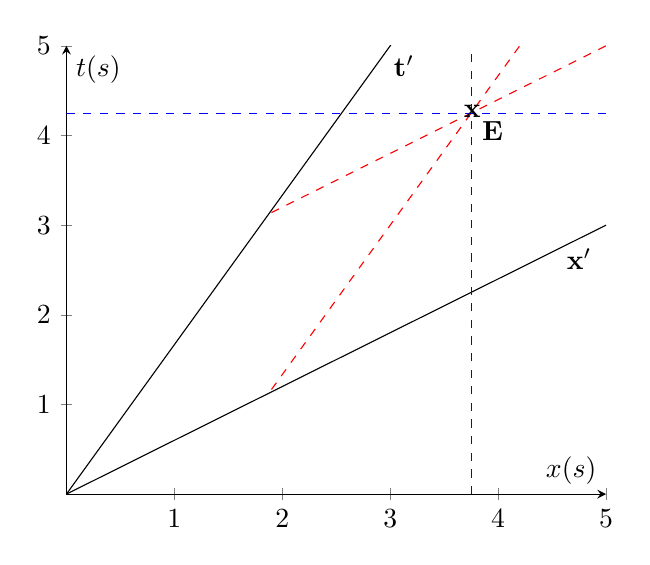
\begin{tikzpicture}
  \begin{axis}[xmin=0, xmax=5, ymin=0, ymax=5, axis x line=middle, axis y line=middle,
    xlabel = \(x(s)\),
    ylabel = \(t(s)\)
    ]
    \addplot[domain=1.9:5, dashed, red]{5/3*x -2} node[pos=0.6](eventt){};
    \addplot[domain=1.9:5, dashed, red]{3/5*x +2} node[pos=0.9](eventx){};
    \addplot[domain=0:5]{5/3*x} node[pos=0.6](tprime){};
    \addplot[domain=0:5]{3/5*x} node[pos=0.95](xprime){};
    \addplot[domain=0:5, dashed, blue]{4.25};
    \addplot[domain=0:5, dashed, blue] coordinates {(3.75, 0) (3.75, 5)};
    \node[below right] at (eventt) {$\mathbf{E}$};
    \node[] at (eventt) {$\mathbf{x}$};
    \node[below] at (tprime) {$\mathbf{\quad t'}$};
    \node[below] at (xprime) {$\mathbf{x'}$};
  \end{axis}
\end{tikzpicture}
\end{center}
Here the blue lines give us the $S$ space time coordinates, and the red lines give us the $S'$ space time coordinates.

\subsection{Lorentz Contraction}
From Lorentz we see that lengths can vary depending on reference frame. Since the endpoints of the object are at rest in rest frame,
the measurement of length is independent of $\Delta t$. If we let $\Delta x = L_{0}$, where $L_{0}$ is the length of an object in its
rest frame, we have:
\begin{align}
  L_{0} = \gamma L
\end{align}
The rest length $L_{0}$ is also often called the proper length. Since $\gamma > 1$ always, objects will always be forshortened in the
direction of motion compared to their proper length.

\subsection{Velocity Transformation}
Now that we have transformation equations for $x$ and $t$ we can combine them to find
an equation relating $v$ and $v'$. Taking $\frac{x'}{t'}$ and simplifying:
\begin{align}
  v' = &\frac{v - \beta}{1 - v \beta}\\
  &\text{or}\\
  v = &\frac{\beta + v'}{1 + v' \beta}
\end{align}
These are known as the Einstein velocity addition eqauations.
\section{Relitivistic Dynamics}

\subsection{The Four-Vector}
We need a definition of momentum that is consistant with SR. Enter the Four-Vector representation of momentum, typically denoted as $p^{\mu}$.
\begin{align*}
  &p^{\mu}= \begin{bmatrix} E \\ \vec{p} \end{bmatrix}\\
  \\
  &p^{\mu}= \begin{bmatrix} E \\ \vec{p}_{x} \\ \vec{p} _{y}\\ \vec{p}_{z} \end{bmatrix}\\
\end{align*}
Four-Vectors use tensor notation, where the upper greek letter indicates an indicie, not an exponent. In this case, $\mu$ ranges from
$\{0, 1, 2, 3\}$. The zeroeth comonect is the time component, in this case its relativistic energy. An objects relativistic energy is
defined as $\gamma m_{0}$, where $m_{0}$ is the rest mass of the object, the mass as measured in a reference frame where it is at rest.
The 1st through 3rd components are the space components, here the relativistic momentum $\gamma m_{0} v$. It is for this reason that
the energy of an object is sometimes refered to as its relativistic mass $m_{rel}$, meaning $p = m_{rel}v$, an intiutive analog of
newtonian momentum. This has fallen out of fashion.

Pluging in the definitions of energy and momentum into our 4-momentum we get the following. Note that for one dimensional problems the
$y$ and $z$ components can be dropped.
\begin{align}
  &p^{\mu}= \begin{bmatrix} \gamma m_{0} \\ \gamma m_{0} \vec{v} \end{bmatrix}
\end{align}

4-Momentum is consereved just like newtonian momentum. Once the final momentum of an
object is determined after a collision, we can extract information about the object
from its 4-momentum. First, to get mass:
\begin{align*}
  E^{2} - |p|^{2} &= \gamma^{2} m_{0}^{2} - \gamma^{2} m_{0}^{2} |v|^{2}\\ \\
  E^{2} - |p|&^{2} = \gamma^{2}m_{0}^{2} (1 - |v|^{2})\\
\end{align*}
Recall the deffinition of $\gamma$:
\begin{align*}
  \gamma^{2} = &\frac{1}{1-|v|^{2}}\\ \\
  E^{2} - &|p|^{2} = m_{0}^{2}
\end{align*}
Therefore:
\begin{align}
  m_{0} = \sqrt{E^{2} - p^{2}}
\end{align}
Notice that we can divide the momentum by energy to get our velocity:
\begin{align}
  &v_{i} = \frac{p_{i}}{E}
\end{align}
If we consider light, which has no rest mass, using eq(20) we see that $E_{\gamma}=p_{\gamma}$. Therefore, the 4-momentum of light is:
\begin{align}
  p^{\mu}_{\gamma} = \begin{bmatrix} E \\ E \end{bmatrix}
\end{align}

Does mass increase as you travel closer to the speed of light? The answer depends on how you define mass. If you
define mass as the amount of stuff in an object, then no. However, if you define it as an objects resistance to
changes in its motion, ie as inertia, then yes, though this is it seen as out of fashion to refer to mass this way
in this context. Cleary, Newton's second law as \(\vec{F}=m\vec{a}\) does not work in the context of relativity.
However, the form \(\vec{F}=\dot{\vec{p}}\) does hold when \(\vec{p}=p_{i}\), the relativistic momentum. When we
take the derivative we get:
\[
  \vec{F}= \gamma m_{0}\dot{\vec{v}}+\dot{\gamma}m_{0}\vec{v}
\]
Where \(m_{0}\) is the rest mass. To find \(\dot{\gamma}\):
\[
  \frac{d\gamma}{dt}=\frac{d\gamma}{dv}\frac{dv}{dt}
\]
Where \(v\) is the speed, not velocity:
\[
  \dot{v}=\frac{d}{dt}\sqrt{\vec{v}\cdot\vec{v}}=\frac{\vec{v}\cdot\vec{a}}{v}
\]

\end{document}
